\documentclass[aspectratio=169,hyperref={pdfpagelabels=false}]{beamer}
\input{preamble.tex}

\subtitle{\normalsize{Industrial IoT for Digitization of Electronis Assets}}
\title{Kalman Filter Estimation and Inflow Prediction}

\setdepartment{DTU Wind and Energy System}
\setcolor{blue}
\captionsetup{font=scriptsize}
\begin{document}
\inserttitlepage

%B SLIDE 0
\begin{frame}{Agenda}
  \begin{itemize}
    \item Estimate the Unmeasured Inflow using The Kalman Filter 
  \end{itemize}
\end{frame}

\begin{frame}
  \frametitle{}
      \begin{block}{State Equation}
        \begin{align*}
          \mathbf{x}_{k+1} &= \mathbf{A}_k \mathbf{x}_k + \mathbf{B}_k \mathbf{u}_k + \mathbf{G}_k \mathbf{w}_k \\
          \mathbf{z}_k &= \mathbf{H}_k \mathbf{x}_k + \mathbf{v}_k 
      \end{align*}
        \end{block}
        \begin{columns}
          \column{0.5\textwidth} % First column
          \begin{itemize}
              \item[-] \(\mathbf{x}_k\): State vector at time \(k\).
              \item[-] \(\mathbf{A}_k\): State transition matrix.
              \item[-] \(\mathbf{B}_k\): Control-input matrix.
              \item[-] \(\mathbf{G}_k\): Noise transformation matrix.
              
          \end{itemize}
          
          \column{0.5\textwidth} % Second column
          \begin{itemize}
            \item[-] \(\mathbf{z}_k\): Measurement at time \(k\).
            \item[-] \(\mathbf{H}_k\): Observation matrix.
            \item[-]  \(\mathbf{w}_k\): Process noise
            \item[-] \(\mathbf{v}_k\): Measurement noise
        \end{itemize}
          \end{columns}


        \end{frame}

  
  \begin{frame}
  \frametitle{Noise Characteristics and Assumptions}
      \begin{itemize}
          \item Process noise \(\mathbf{w}_k\) and measurement noise \(\mathbf{v}_k\) are typically independent.
          \item Both noises are modeled as white noise (constant spectral density, uncorrelated in time).
          \item \(\mathbf{G}_k\) scales or transforms process noise to align with the state space.
      \end{itemize}
  \end{frame}

\begin{frame}{}
  $x_0 \sim \tilde{x_0}$ and covariance $P_0$
  \begin{block}{Covariance, of the process noise $w_k$ and the measurement noise $v_k$}
    \begin{align*}
      \mathbb{E}\Biggl [
        \begin{pmatrix}
        w_k \\
        v_k
        \end{pmatrix}
        \begin{pmatrix}
          w_{\ell}' & v_{\ell}'
          \end{pmatrix}
        \Biggr ] = \Biggl [ \begin{matrix}
          Q_k & 0\\
          0 & R_k 
          \end{matrix} \Biggr ] \delta_{kl}
    \end{align*}
  \end{block}
\begin{itemize}
  \item The resulting matrix has zeros off diagional, uncorrelated error with each other.
  \item The $\delta_{kl}$ means that the autocorrelation is non-zero on for $l=k$, thus they are independent in time (independece of sample in white noise)
\end{itemize}
\end{frame}

\begin{frame}
  \begin{figure}
    \centering
    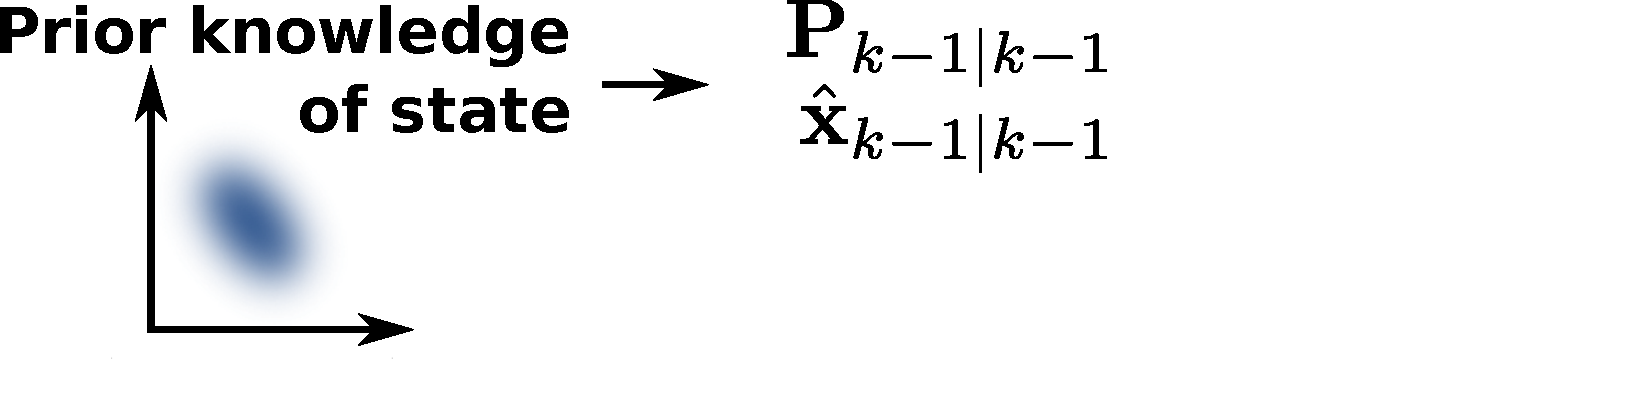
\includegraphics[width=0.9\linewidth]{img/3.pdf}
    \caption{\\ Priori Knowledge from the previous measurements}
  \end{figure}
\end{frame}

\begin{frame}{Prediction Phase: Step 1.1}
  Let's start by considering the state update (no new measurement)
  \begin{block}{Predicted State Estimate (a priori)}
  \begin{align*}
    \boxed{\hat{x}_{k|k-1} = F_{k} \hat{x}_{k-1|k-1} + B_{k}u_{k}}
  \end{align*}
  \begin{itemize}
    \item[-] $\mathbf{\hat{x}_{k|k-1}} \rightarrow$ estimate of x at time $k$ given $k-1$.
    \item[-] $\mathbf{\hat{x}_{k-1|k-1}} \rightarrow$ all the estimation up to $k-1$ given $k-1$ observations.
    \item[-] $\mathbf{Bu_{k-1}} \rightarrow$ deterministic input.
  \end{itemize}
  \end{block}
\end{frame}


\begin{frame}{Prediction Phase: Step 1.2 }
  
  \begin{block}{Predicted Estimate Covariance (\textit{a priori})}
    \begin{align*}
      \hat{P}_{k|k-1} &= F_{k}P_{k|k-1}F_{k}^T + Q_{k}
      \end{align*}
  \begin{itemize}
    \item[-] $\mathbf{P_{k|k-1}} \rightarrow$ predicted state covariance matrix at time $k$ based on $P_{k-1}$.
    \item[-] $\mathbf{F_{k}}$ is the state transition matrix
    \item[-] $\mathbf{Q_k}$ is the covariance matrix of the process noise
  \end{itemize}
  \end{block}
\end{frame}

\begin{frame}
  \begin{figure}
    \centering
    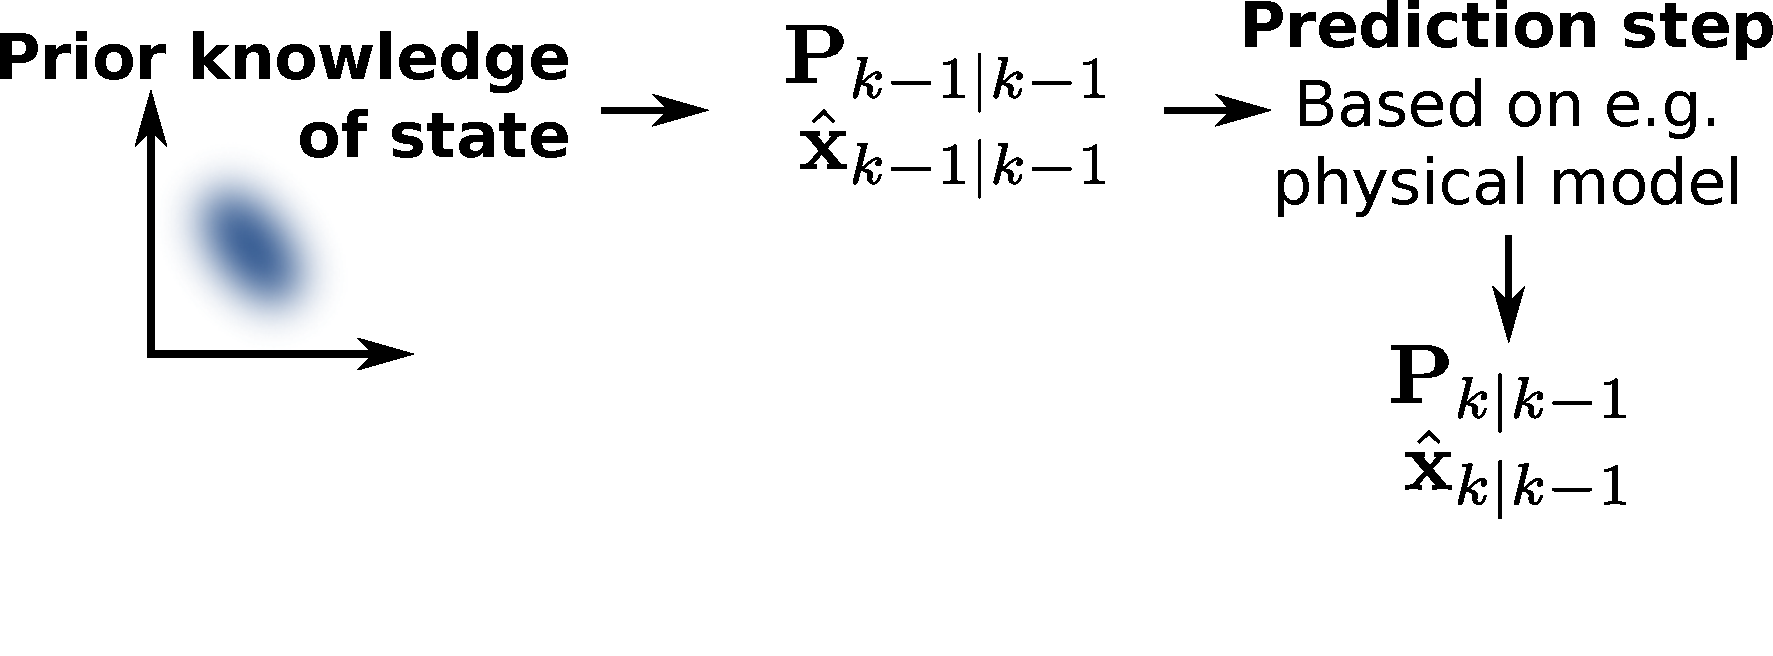
\includegraphics[width=1\linewidth]{img/4.pdf}
  \end{figure}
\end{frame}

\begin{frame}
  \frametitle{Update Phase: Step 2.1}
  New measurement available
  \begin{block}{Measurement Update Equation}
    \begin{align*}
      y_{k} &= z_{k} - H_{k}\hat{x}_{k|k-1}
      \end{align*}
      \begin{itemize}
        \item[-] $\mathbf{y_k} \rightarrow$ represents the measurement at time step $k$
        \item[-] $\mathbf{z_k}$ is the predicted measurement at time step $k$.
        \item[-] $\mathbf{H_k}$ is the observation matrix at time step $k$.
      \end{itemize}
  \end{block}
\end{frame}

\begin{frame}
  \frametitle{Update Phase: Step 2.2}
  New measurement available
  \begin{block}{Innovation of Covariance Matrix }
    \begin{align*}
      S_{k|k-1} &= H_{k}\hat{P}_{k|k-1}H_{k}^T + R_{k}
      \end{align*}
      \begin{itemize}
        \item[-] $\mathbf{y_k} \rightarrow$ represents the measurement at time step $k$
        \item[-] $\mathbf{z_k}$ is the predicted measurement at time step $k$.
        \item[-] $\mathbf{H_k}$ is the observation matrix at time step $k$.
      \end{itemize}
  \end{block}
\end{frame}


\begin{frame}
  \frametitle{Update Phase: Step 2.3}
  New measurement available
  \begin{block}{Kalman Gain}
    \begin{align*}
      S_{k|k-1} &= H_{k}\hat{P}_{k|k-1}H_{k}^T + R_{k}
      \end{align*}
      \begin{itemize}
        \item[-] $\mathbf{y_k} \rightarrow$ represents the measurement at time step $k$
        \item[-] $\mathbf{z_k}$ is the predicted measurement at time step $k$.
        \item[-] $\mathbf{H_k}$ is the observation matrix at time step $k$.
      \end{itemize}
  \end{block}
\end{frame}



\begin{frame}
\frametitle{Update Phase: Step 2.4}
    \begin{block}{Kalman Gain Calculation}
      \begin{align*}
        K_{k} &= \hat{P}_{k|k-1}H_{k}^T S_{k}^{-1} \\
        K_{k} &= \hat{P}_{k|k-1}H_{k}^T(H_{k}P_{k|k-1}H_{k}^T + R_{k})^{-1}
        \end{align*}        
    \end{block}

\end{frame}

\begin{frame}{Update Phase: Step 2.5}
  \begin{block}{Updated State Estimate}
    \[ \hat{x}_{k|k} = \hat{x}_{k|k-1} + K_{k}y_{k} \]
\end{block}
  \begin{block}{Updated Estimate Covariance}
    \begin{align*}
      P_{k|k} = (I - K_{k}H_{k})P_{k|k-1}
    \end{align*}
\end{block}
\end{frame}

\begin{frame}
  \begin{figure}
    \centering
    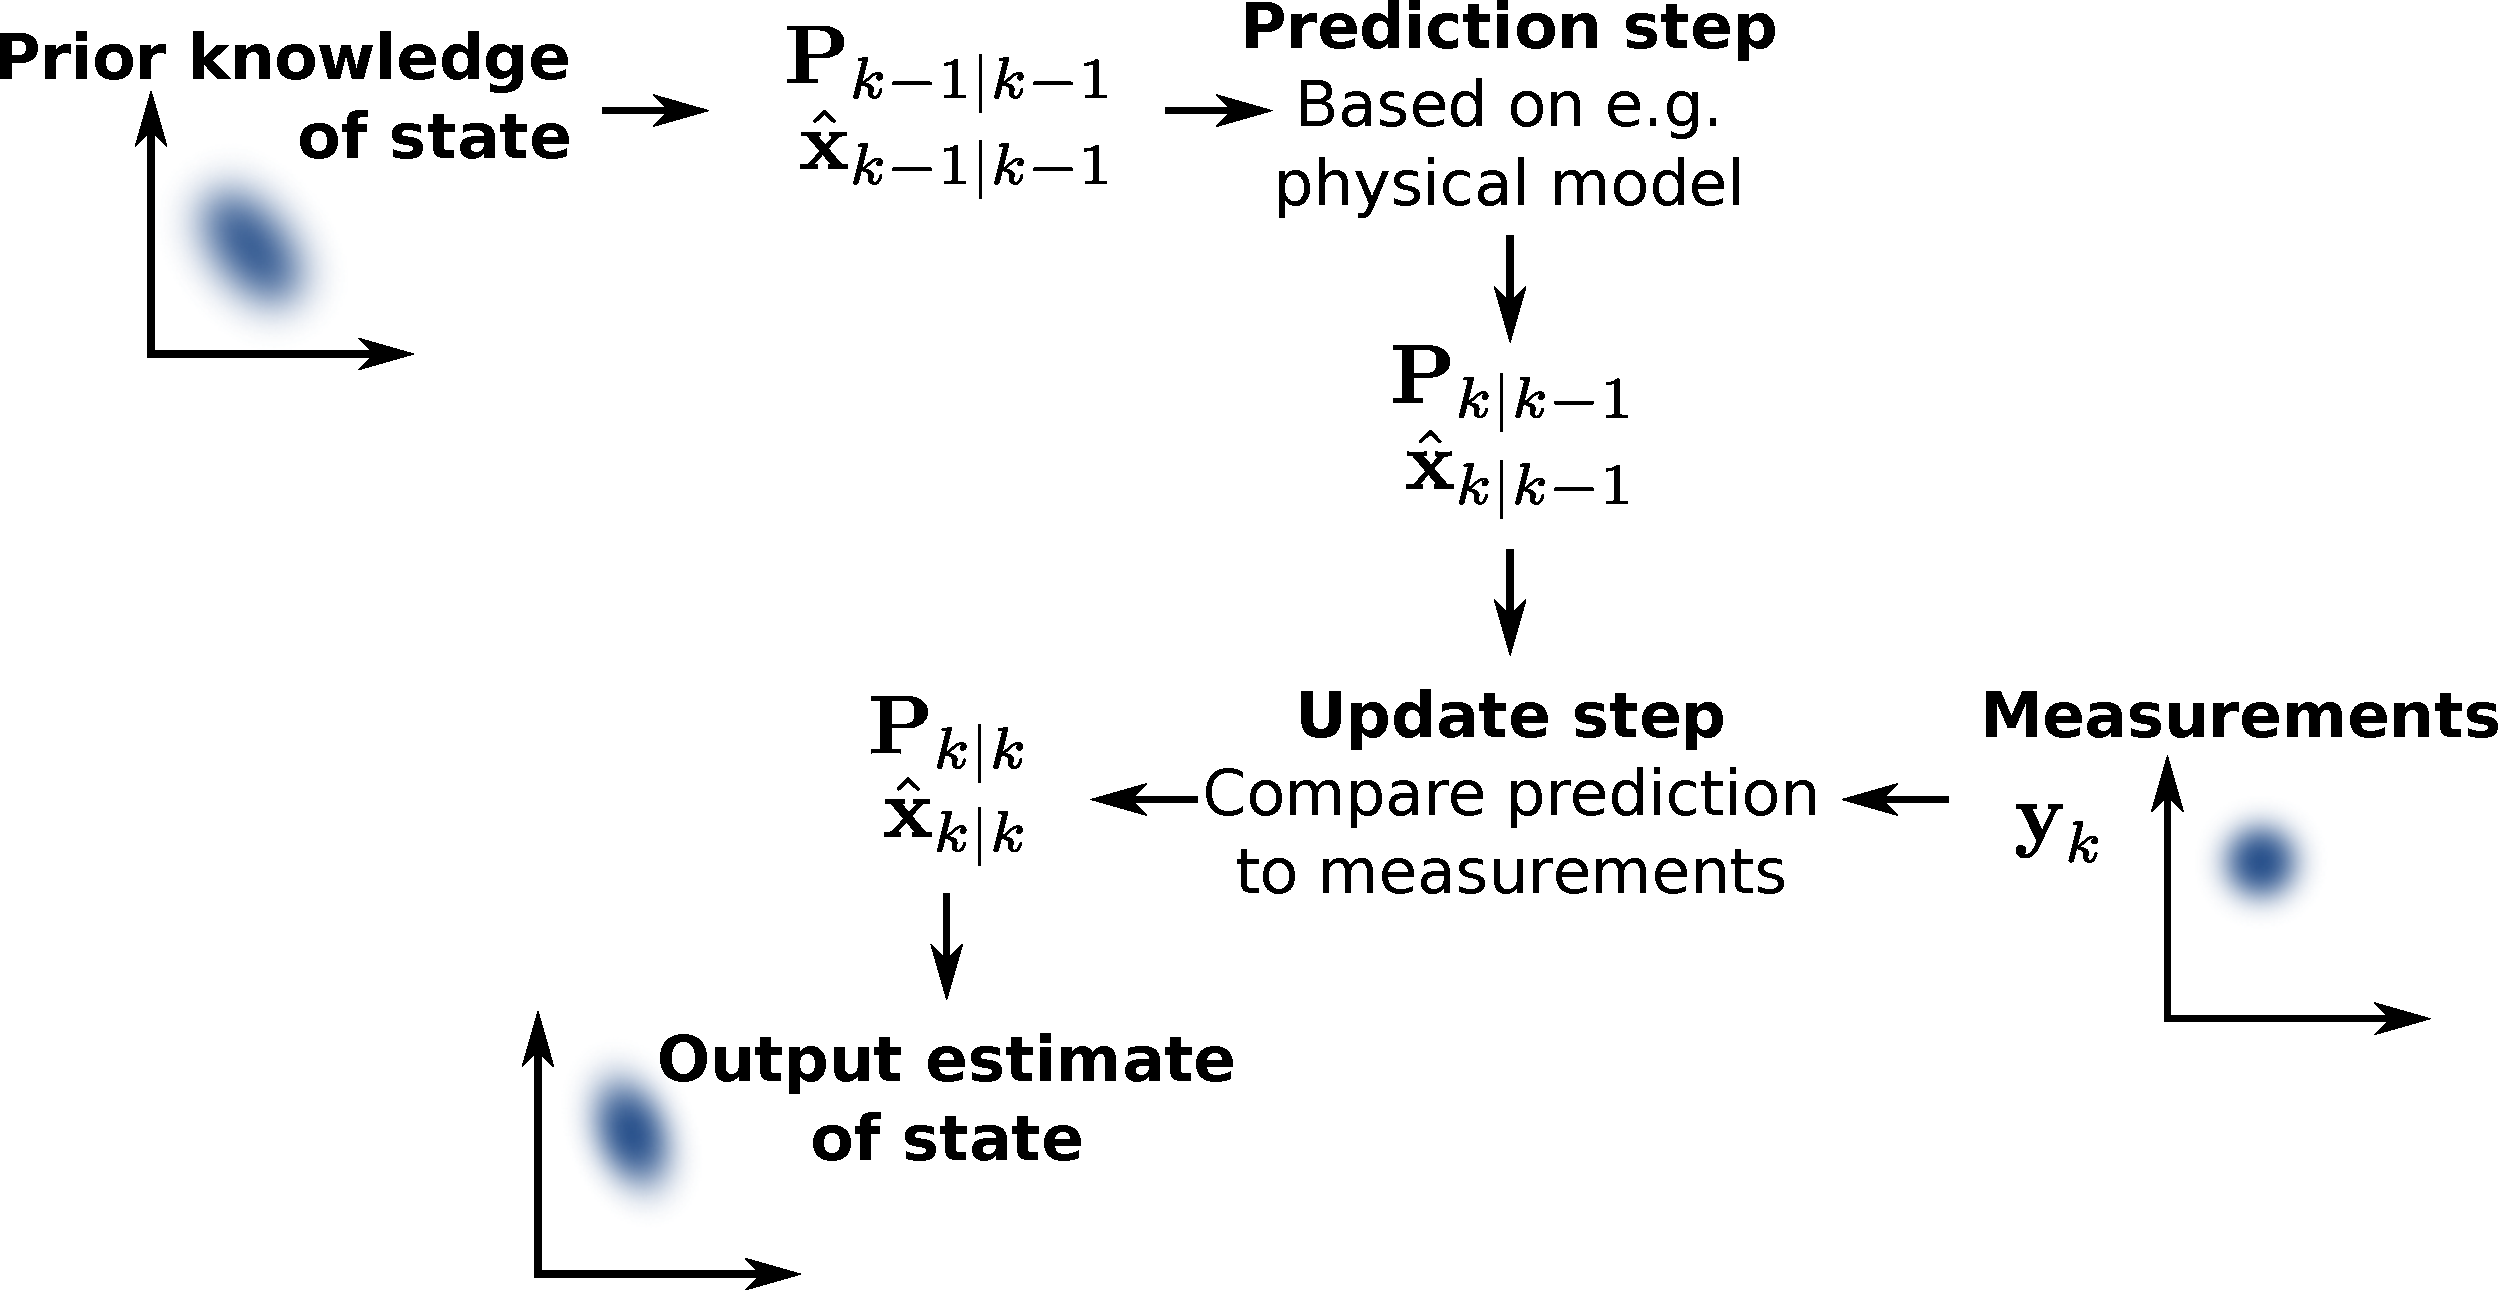
\includegraphics[width=1\linewidth]{img/5.pdf}
  \end{figure}
\end{frame}


\begin{frame}
  \begin{figure}
    \centering
    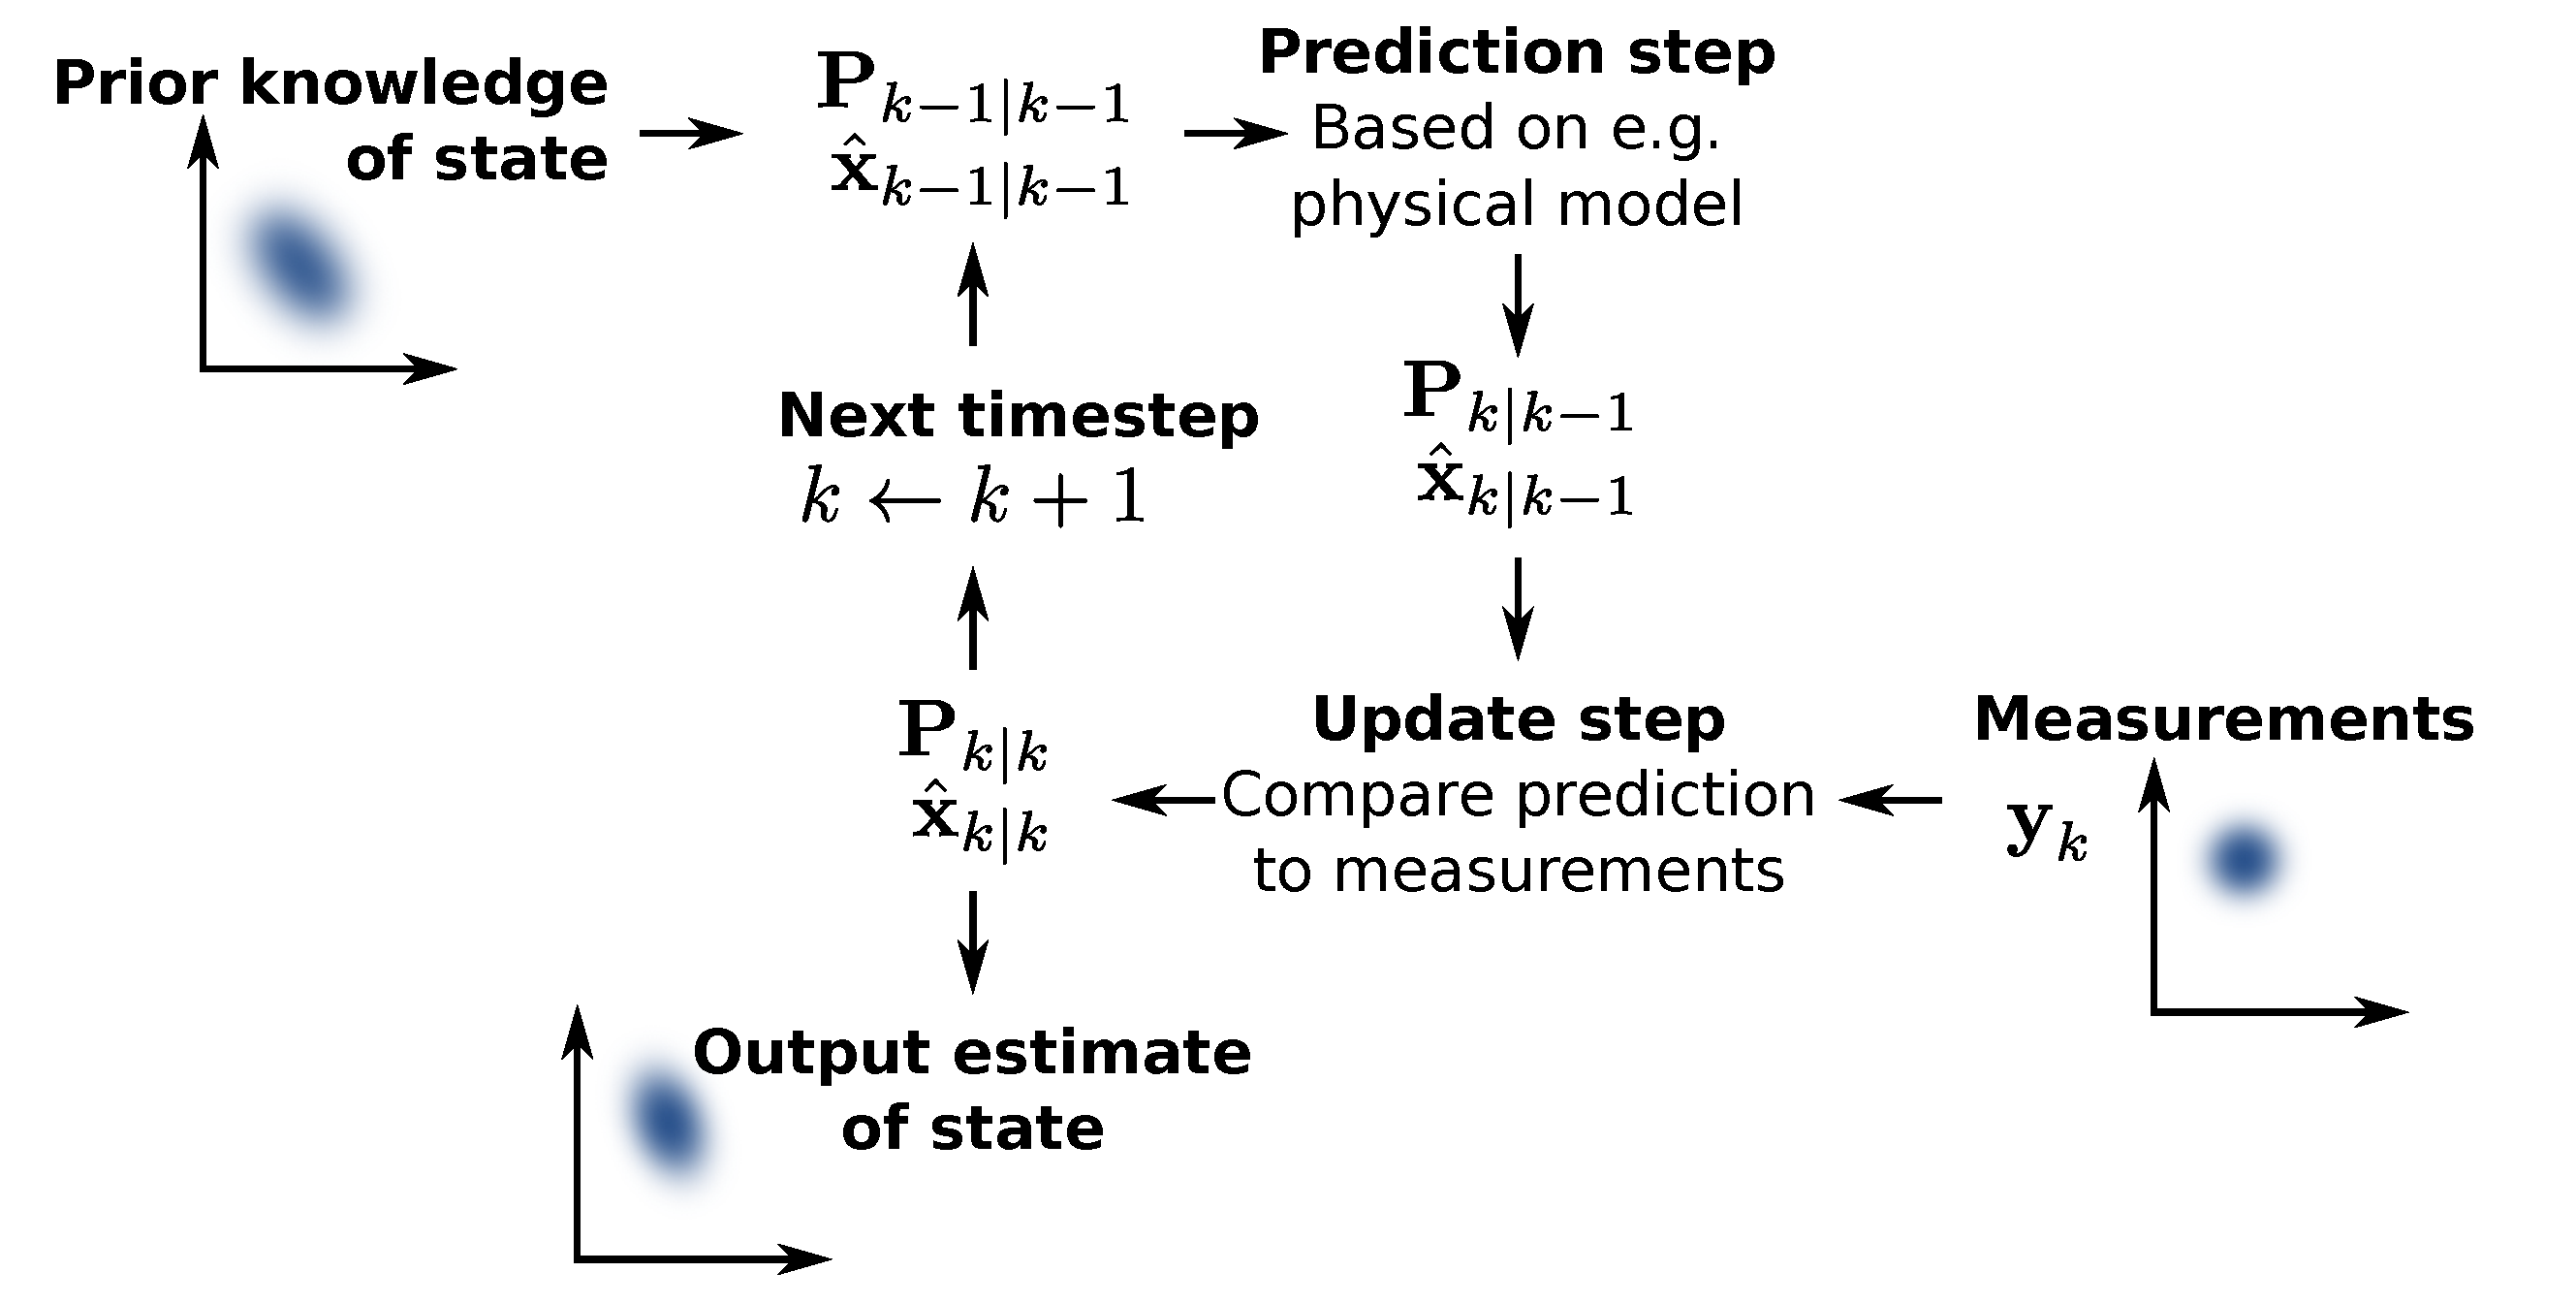
\includegraphics[width=1\linewidth]{img/Basic_concept_of_Kalman_filtering.pdf}
  \end{figure}
\end{frame}


\begin{frame}
  \frametitle{Inflow Estimation of the Wastewater Tank}
      \begin{itemize}
          \item The goal is to estimate the inflow rate (\(Q_{in}\)) in a reservoir system without direct measurements.
          \item Kalman Filter is utilized to estimate \(Q_{in}\) using the water height (\(h\)) and outflow rate (\(Q_{out}\)) measurements.
          \item The estimation is crucial for building the inflow forecast and the controller.
          \item State Variables: Inflow Rate (\(Q_{in}\)), Water Height (\(h\)), Outflow Rate (\(Q_{out}\)).
          \item Measurements: Water Height and Outflow Rate.
      \end{itemize}
  \end{frame}
  
  \begin{frame}
    \frametitle{System Model}
        \begin{itemize}
            \item The continuous-time model is given by the differential equation:
            \[ \frac{dh}{dt} = \frac{t_{sampling}}{A} (Q_{in}(t) - Q_{out}(t)) \]
            \item             
            \begin{align*}
              \frac{dh}{dt} = 0 \longrightarrow  Q_{in}(t) = Q_{out}(t)
            \end{align*}
        \end{itemize}
    \end{frame}

  \begin{frame}
  \frametitle{State Transition Matrix (A)}
      \[ A = \begin{bmatrix} 1 & 0 & 0 \\ \frac{t}{\text{area}} & 1 & -\frac{t}{\text{area}} \\ 0 & 0 & 1 \end{bmatrix} \]
      \begin{itemize}
          \item Describes the system's evolution over time.
          \item \(t\) is the time step, and \(\text{area}\) is a system parameter.
      \end{itemize}
  \end{frame}
  
  \begin{frame}
  \frametitle{Observation Matrix (H) and Measurements}
      \[ H = \begin{bmatrix} 0 & 1 & 0 \\ 0 & 0 & 1 \end{bmatrix} \]
      \begin{itemize}
          \item Maps state variables to measurements.
          \item Observes water height (\(h\)) and outflow rate (\(Q_{out}\)).
      \end{itemize}
  \end{frame}
  
  \begin{frame}
  \frametitle{Process and Measurement Noise}
      \begin{itemize}
          \item Process Noise: Error estimates for \(Q_{in}\), \(h\), \(Q_{out}\).
          \item Measurement Noise: Error in measuring \(h\) and \(Q_{out}\).
      \end{itemize}
  \end{frame}
  
  \begin{frame}
  \frametitle{Initial State and Covariance}
      \begin{itemize}
          \item Initial State: Estimates for \(Q_{in}\), \(h\), \(Q_{out}\).
          \item Covariance: Represents initial uncertainty in state estimates.
      \end{itemize}
  \end{frame}

  \begin{frame}{\normalsize{Python Tutorial: Build The Kalman Filter To Estimate the Inflow}}
    \begin{figure}
      \centering
      \begin{subfigure}[b]{0.3\textwidth}
          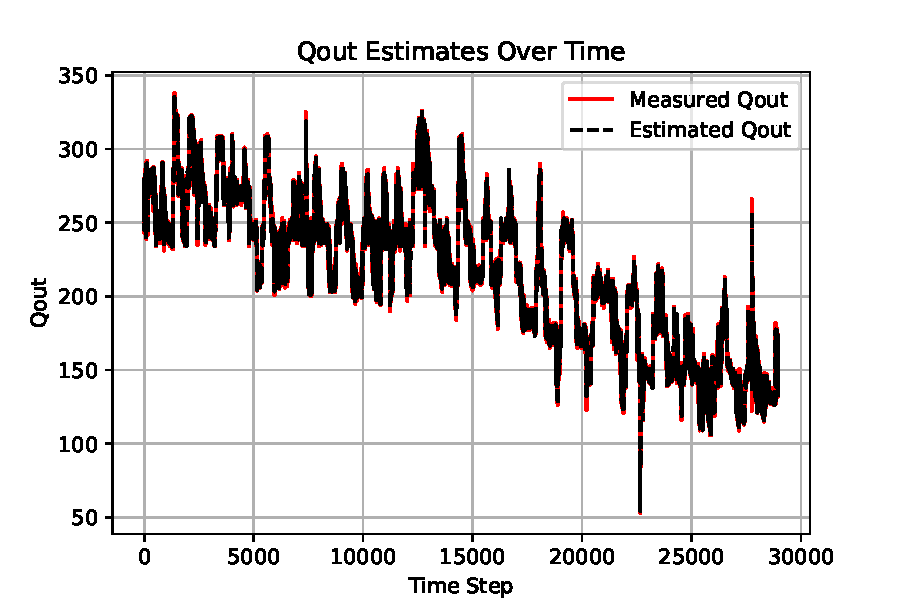
\includegraphics[width=\textwidth]{/home/alqua/Git/Industrial-IoT-For-Digitization-Of-Electronic-Assets/Module 4/img/inflow_estimate_using_KF_3.pdf}
          \caption{Outflow Estimation vs Measurements}
          \label{fig:image1}
      \end{subfigure}
      \hfill
      \begin{subfigure}[b]{0.3\textwidth}
          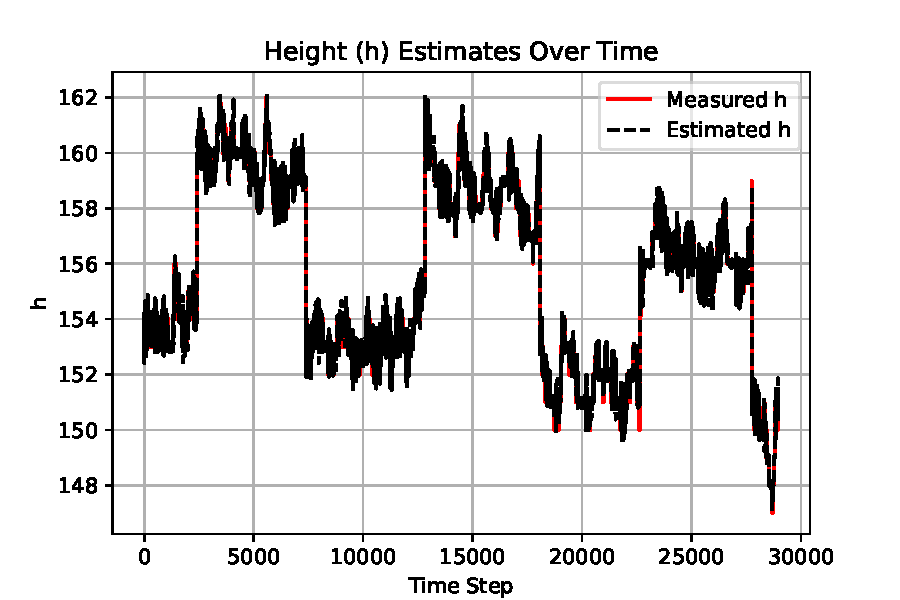
\includegraphics[width=\textwidth]{/home/alqua/Git/Industrial-IoT-For-Digitization-Of-Electronic-Assets/Module 4/img/inflow_estimate_using_KF_2.pdf}
          \caption{Height Estimation vs Measurements}
          \label{fig:image2}
      \end{subfigure}
      \hfill
      \begin{subfigure}[b]{0.3\textwidth}
          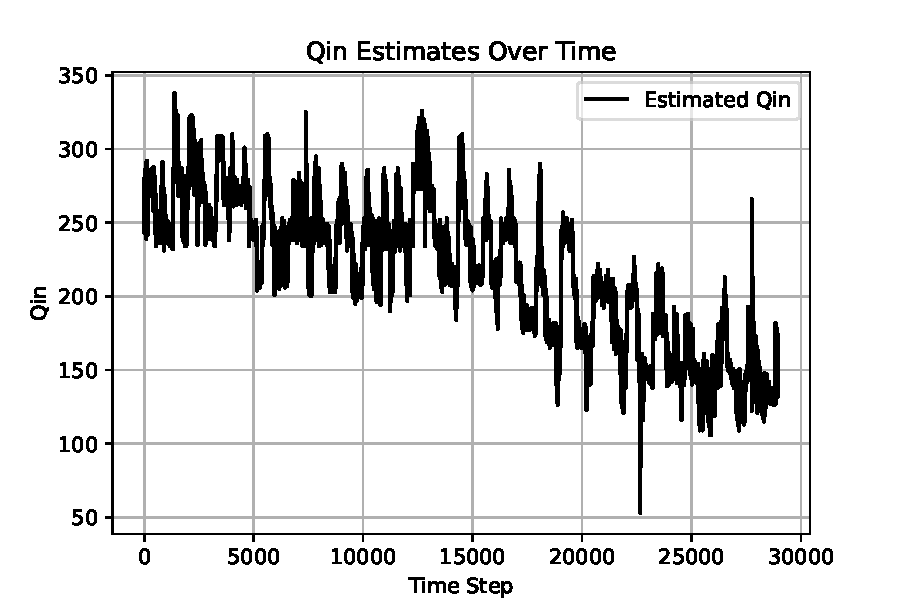
\includegraphics[width=\textwidth]{/home/alqua/Git/Industrial-IoT-For-Digitization-Of-Electronic-Assets/Module 4/img/inflow_estimate_using_KF_1.pdf}
          \caption{Indirect Inflow Estimation}
          \label{fig:image3}
      \end{subfigure}
      \end{figure}
  \end{frame}



\end{document}